\chapter{实验设计}

\section{引言}
进行实验关键是传感器的校准、实现夹爪的力控、相机的校准和识别算法的设计。
本章将介绍实验用到的设备和仪器,传感器的校准和力控的实现方法,
最后用仿真实验验证上文提出方案。

\section{实验装置}
该项目中用到的主要设备有单自由度高速夹爪一个,压力传感器一枚,
信号采集器一个,高速相机一台。实验装置如图 \ref{fig:4-1} 所示。

\begin{figure}[!ht]
  \centering
  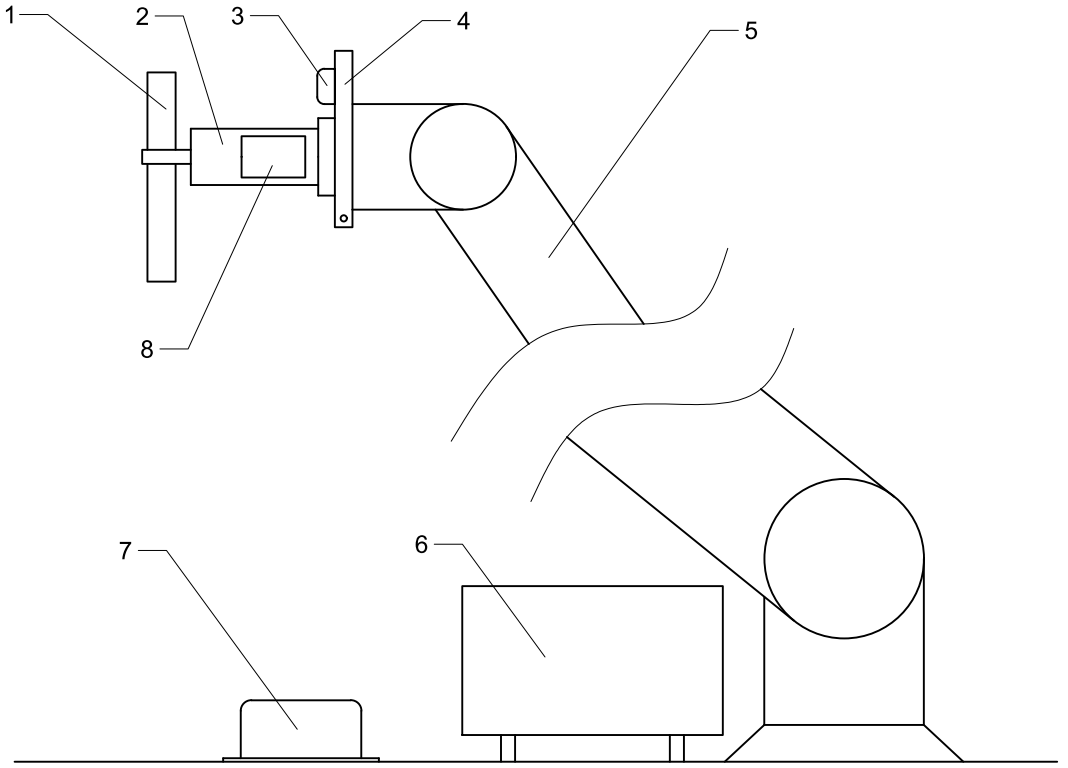
\includegraphics[scale=0.4]{chapter04/pic/4-1}
  \caption{实验装置简图}
  \label{fig:4-1}
  \vspace{-0.3cm}
\end{figure}

\vspace{-10pt}
\begin{center}
  \zihao{-5}
  1---被控物体; 2---高速夹爪; 3---Realsense相机; 4---相机支架; \\
  5---机械臂; 6---机械臂控制箱; 7---夹爪控制器; 8---数据采集卡;
\end{center}

图中相机固定在相机支架上,同高速夹爪一起固定在机械臂末端;
数据采集卡固定在夹爪上;薄膜式压力传感器贴在夹爪内侧,
通过设计的电路与数据采集卡连接。
按照各设备要求连接通信线路,夹爪连接控制器,
控制器和相机均通过 USB 线缆连接上位机;
机械臂用专用线缆连接控制箱,控制箱通过网线连接上位机。

由于本项目中机械臂不需要运动, 所以为了便于实验, 我们简化了实验装置,
使用设计的支架代替机械臂来固定夹具和相机。
我们最终搭建的实验平台的俯视图和侧视图分别如图\ref{fig:exp-1}和图\ref{fig:exp-2}所示,
依照图示方法固定设备后, 连接电路后即可进行实验。

\begin{figure}[!ht]
  \centering
  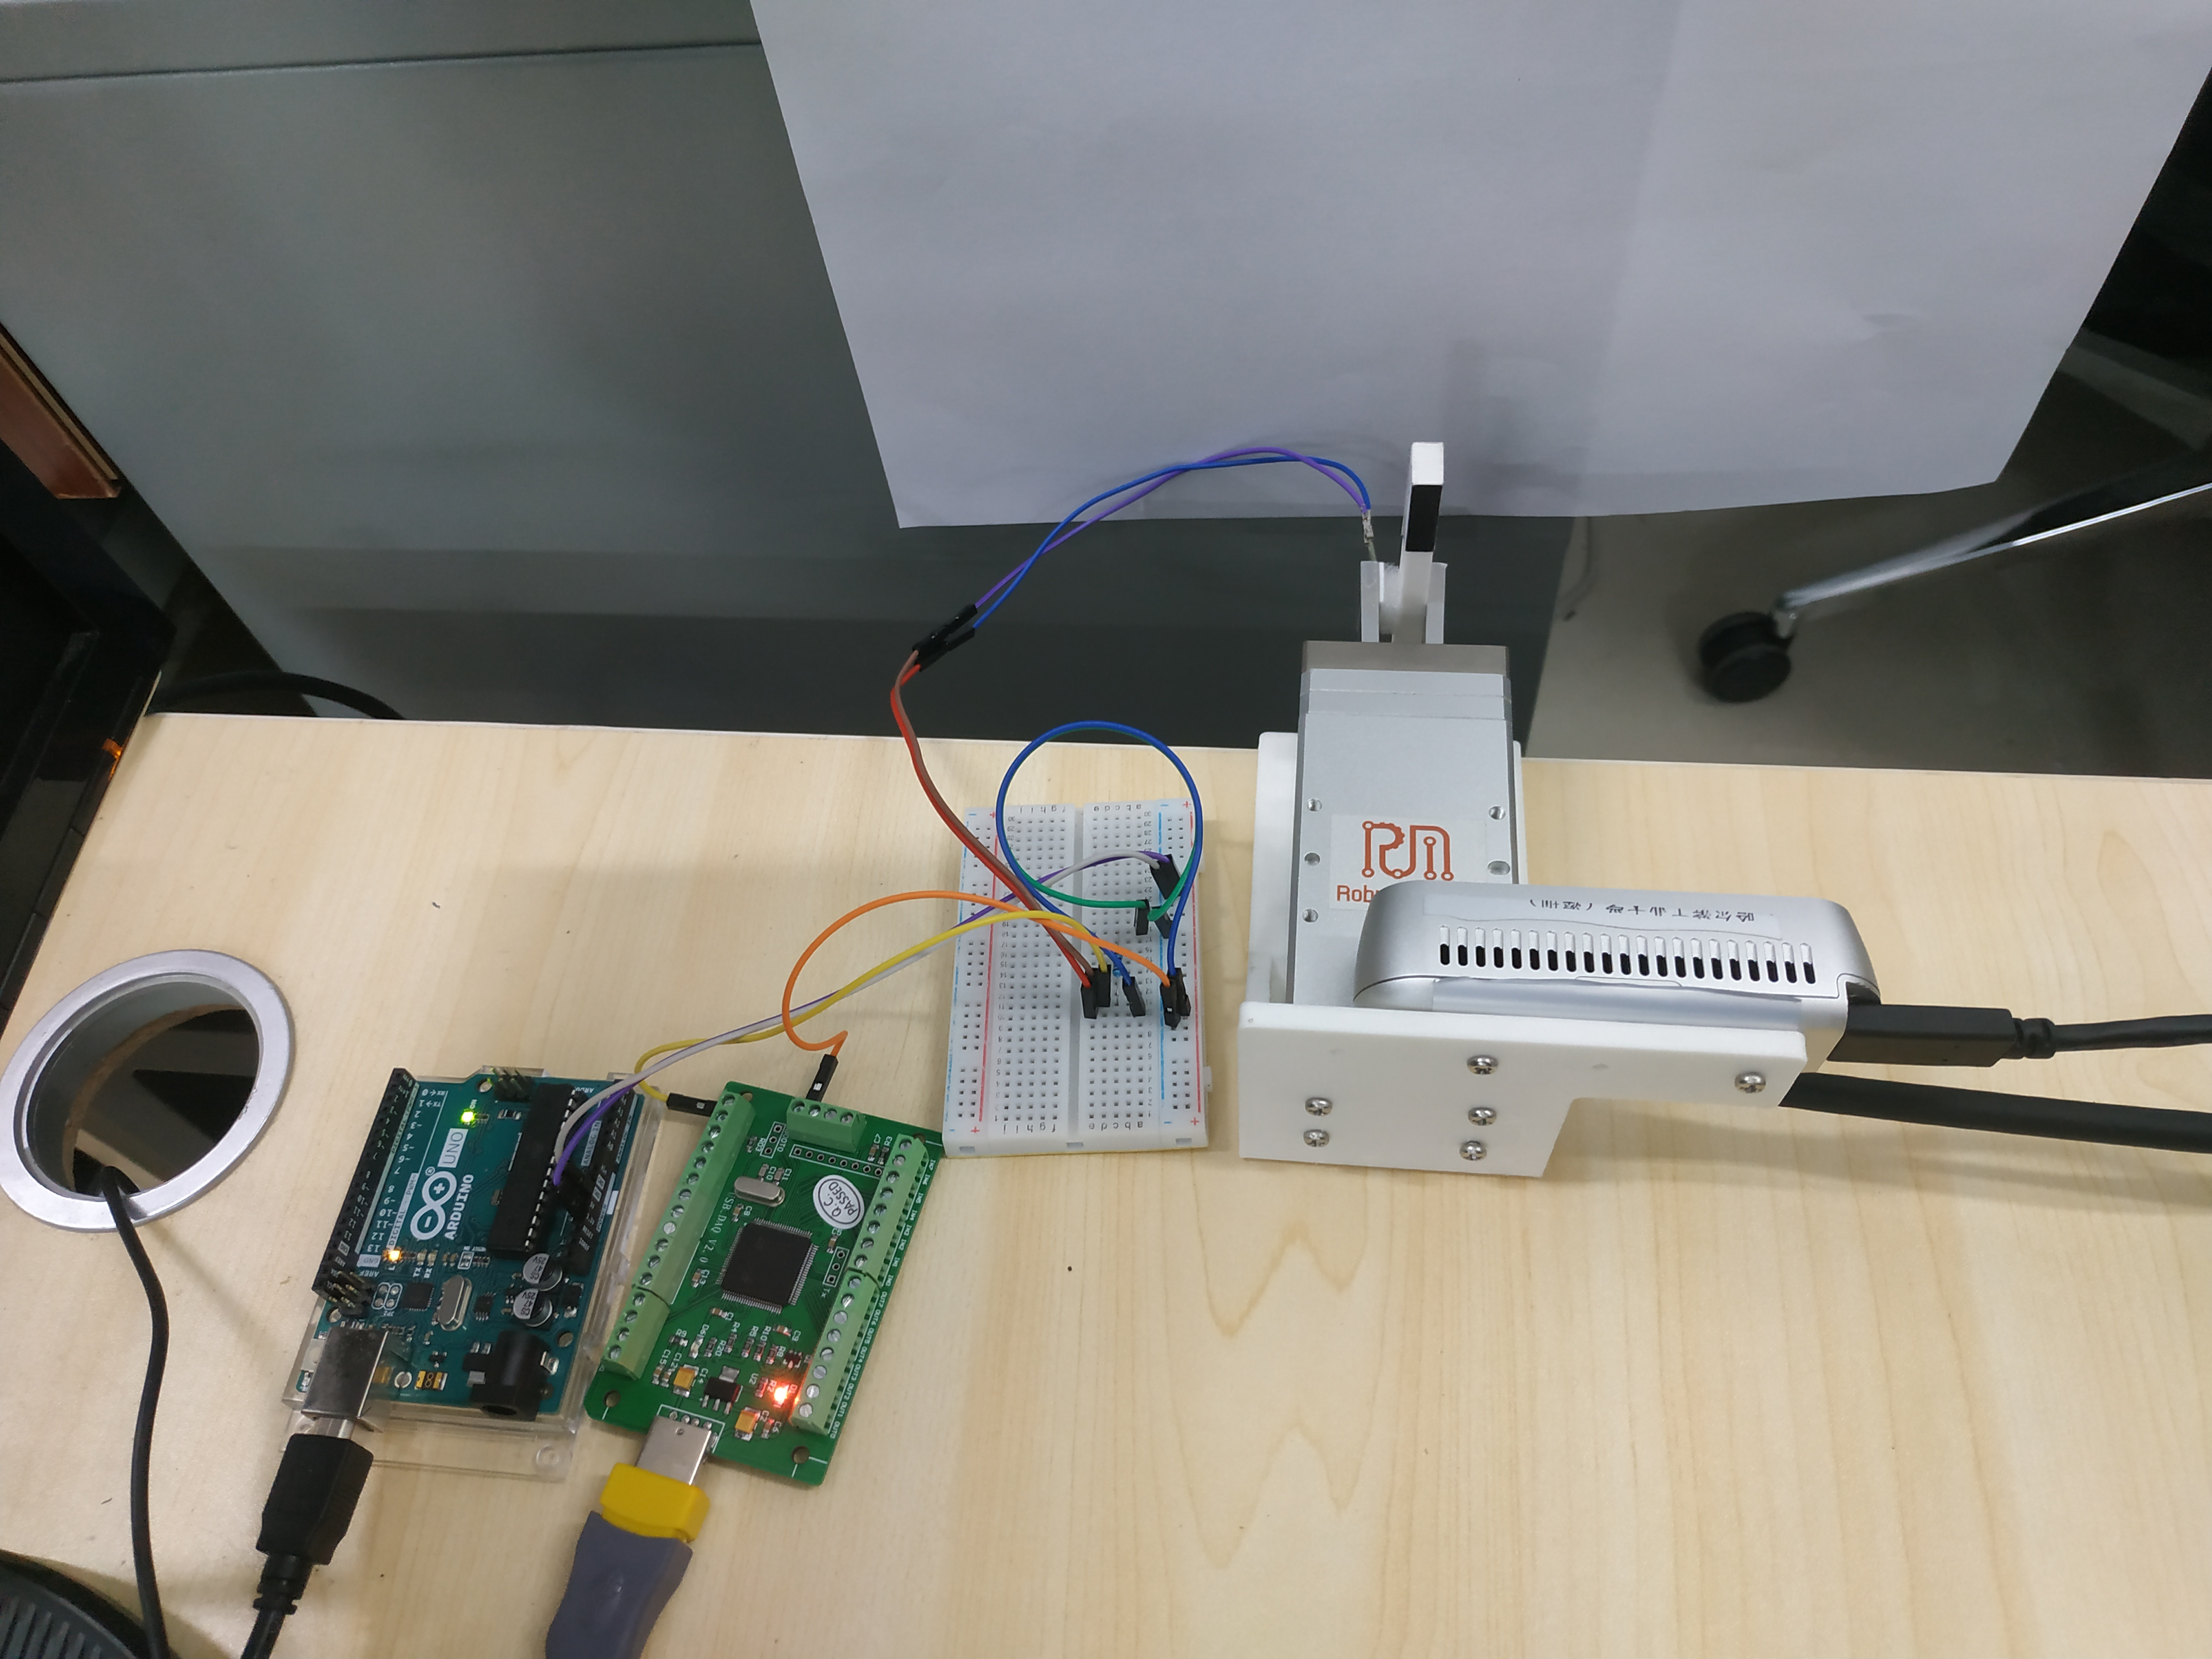
\includegraphics[width=11.3cm]{chapter04/pic/exp-1}
  \caption{\label{fig:exp-1}
    实验平台俯视图}
  \vspace{-0.3cm}
\end{figure}

\begin{figure}[!ht]
  \centering
  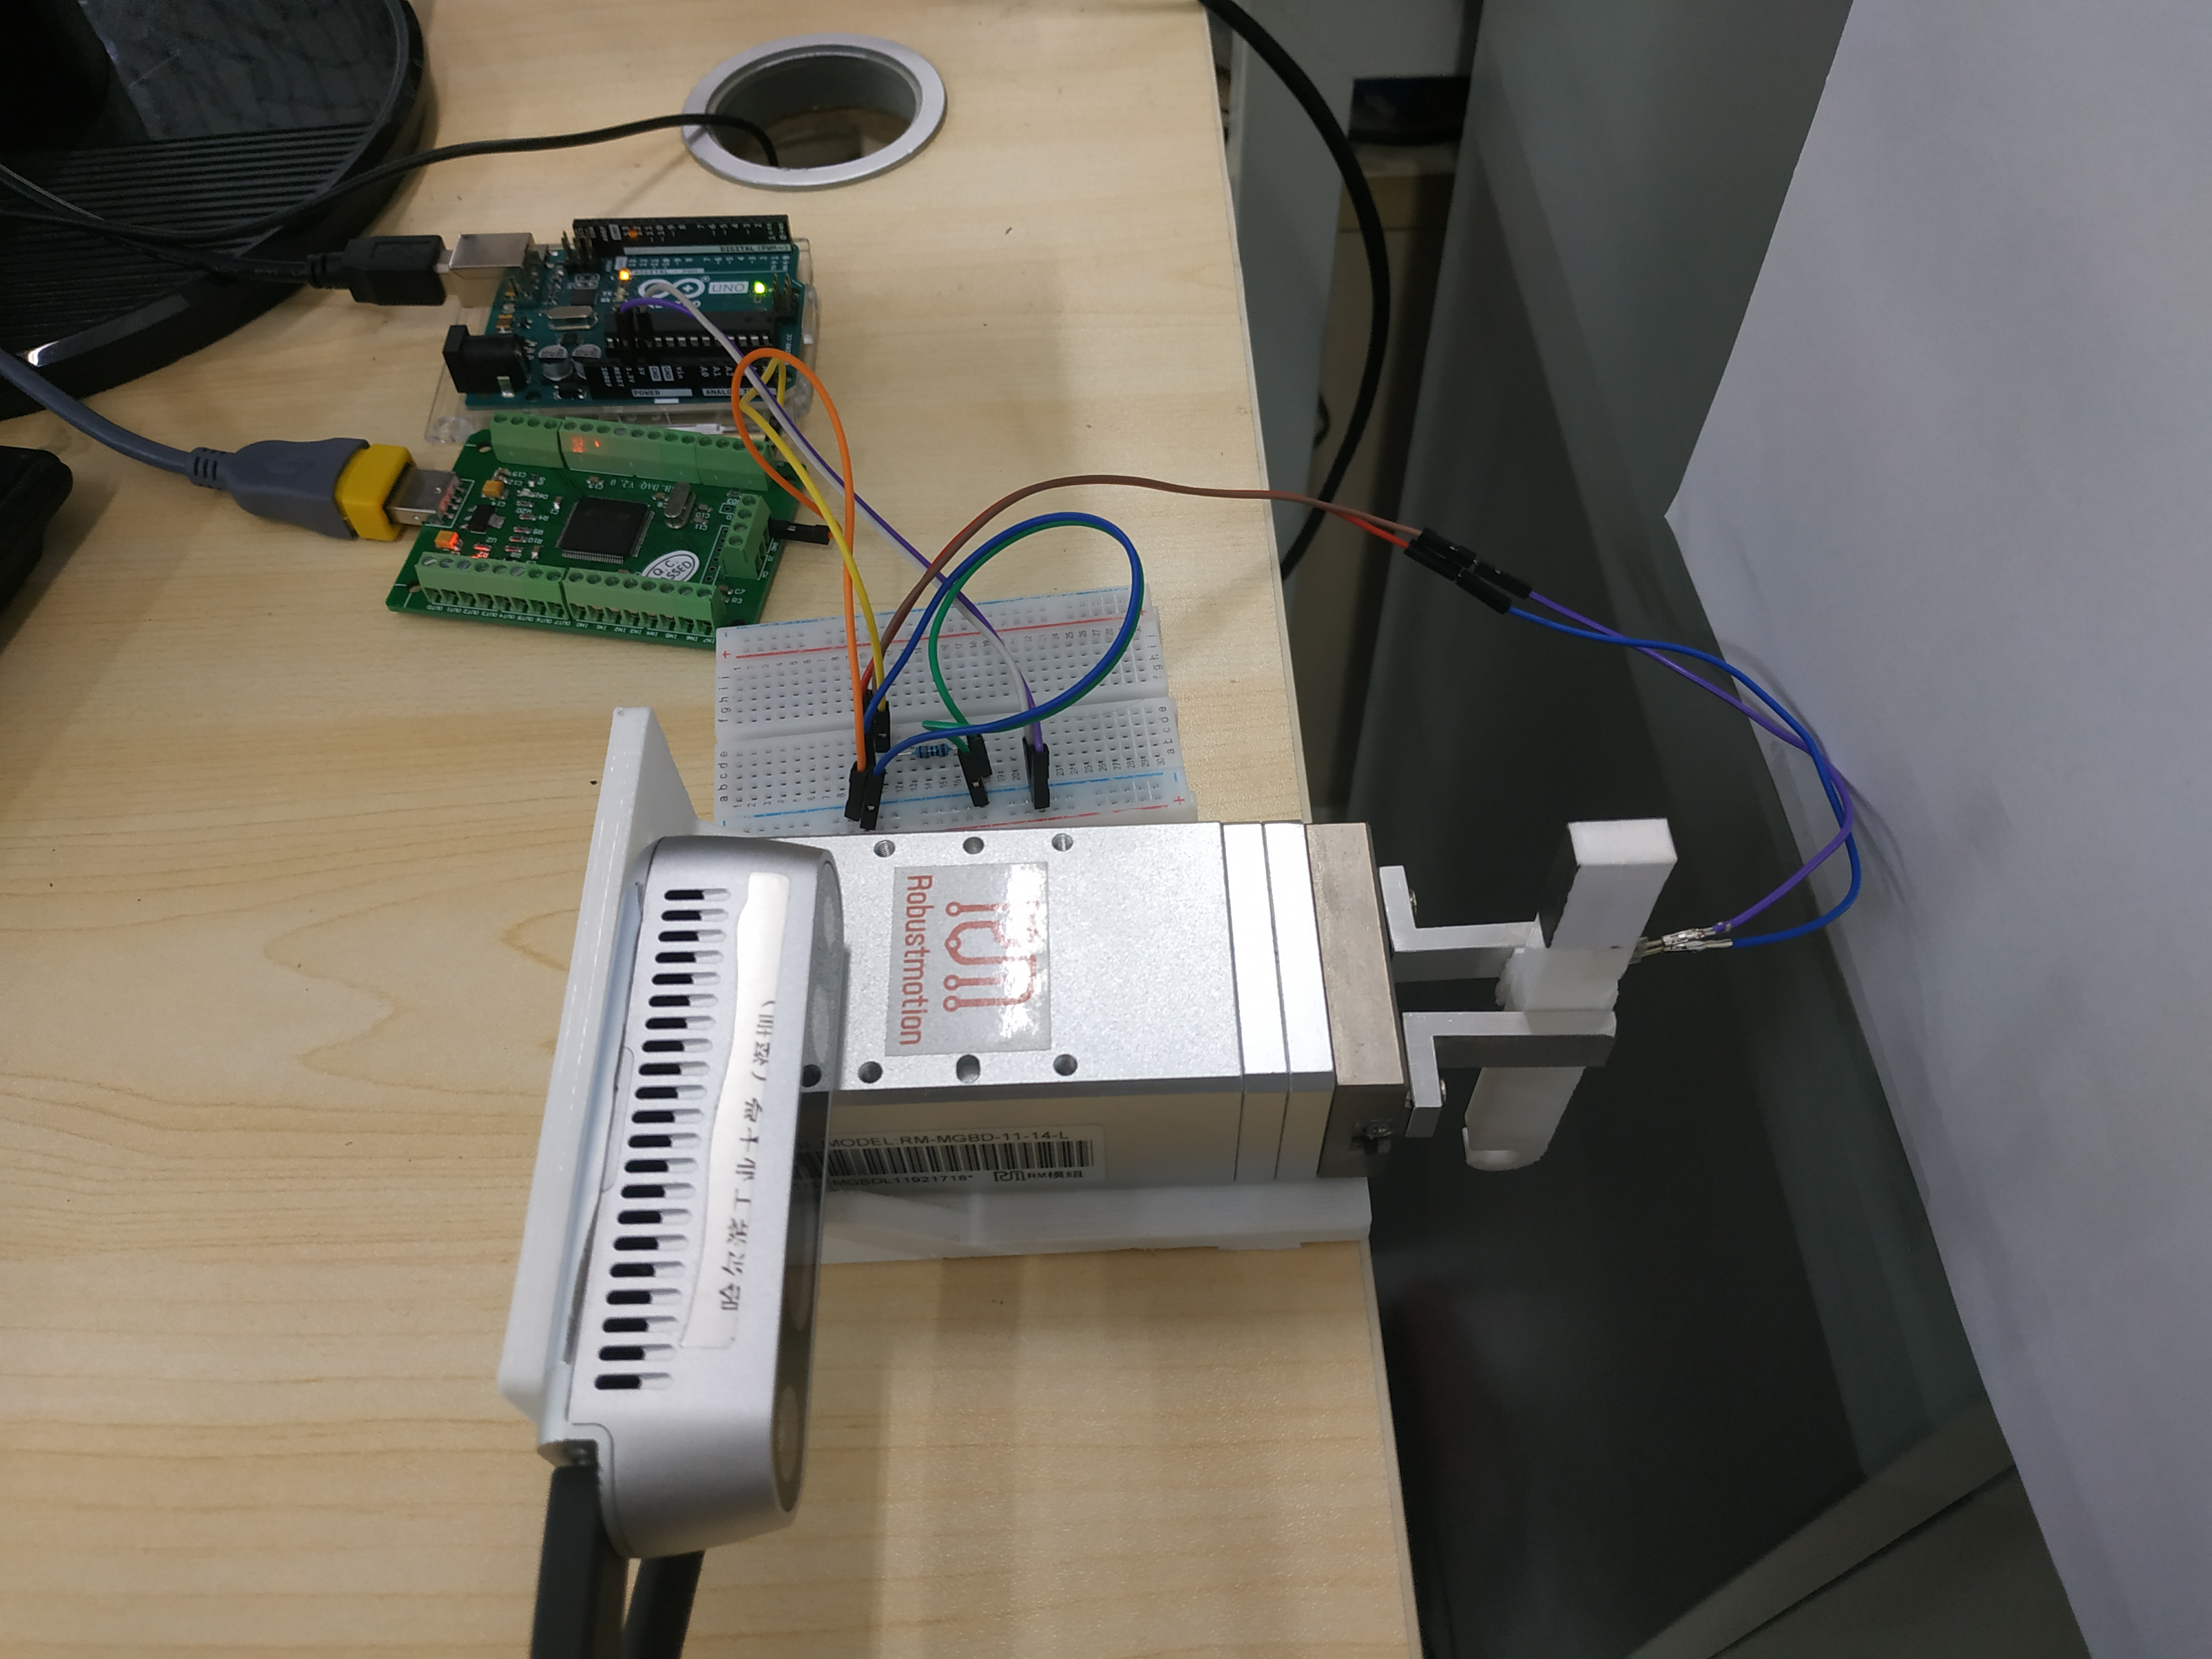
\includegraphics[width=11.3cm]{chapter04/pic/exp-2}
  \caption{\label{fig:exp-2}
    实验平台侧视图}
  \vspace{-0.3cm}
\end{figure}

% \begin{figure}[!h]
%   \centering
%     \subfloat[俯视图]{
%       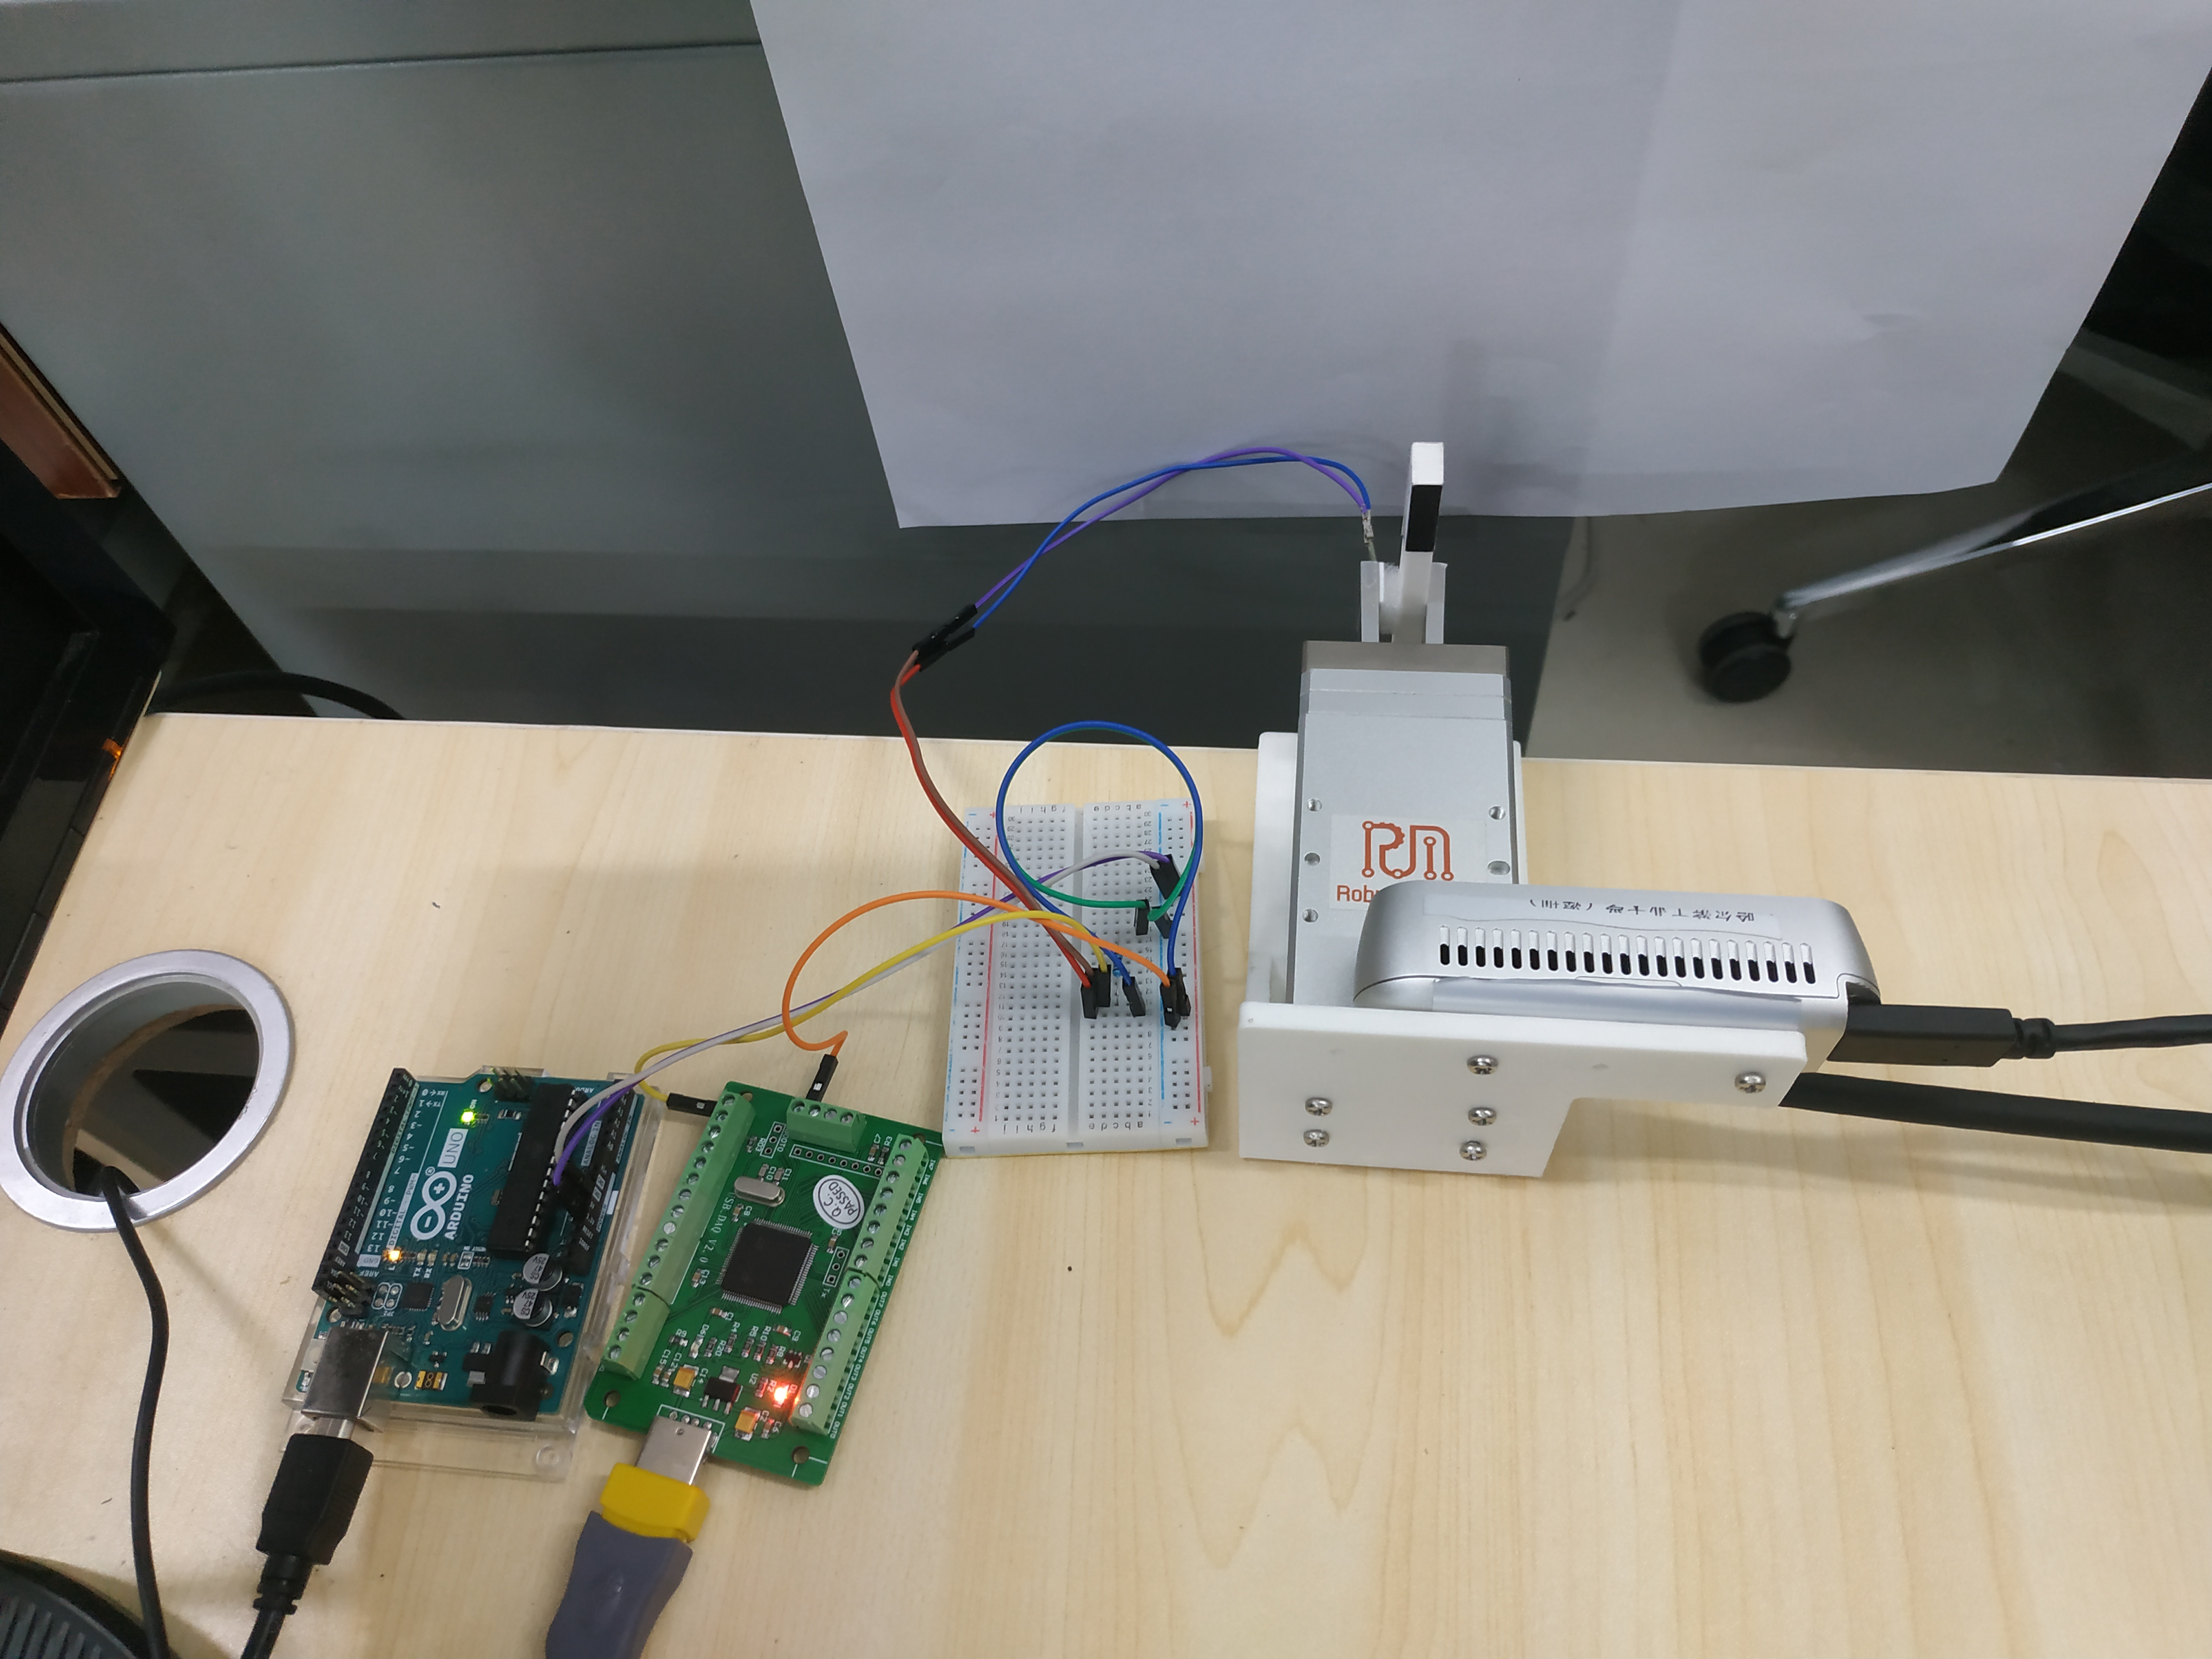
\includegraphics[width=7.2cm]{chapter04/pic/exp-1}
%     }
%     \hspace{0pt}
%     \subfloat[侧视图]{
%       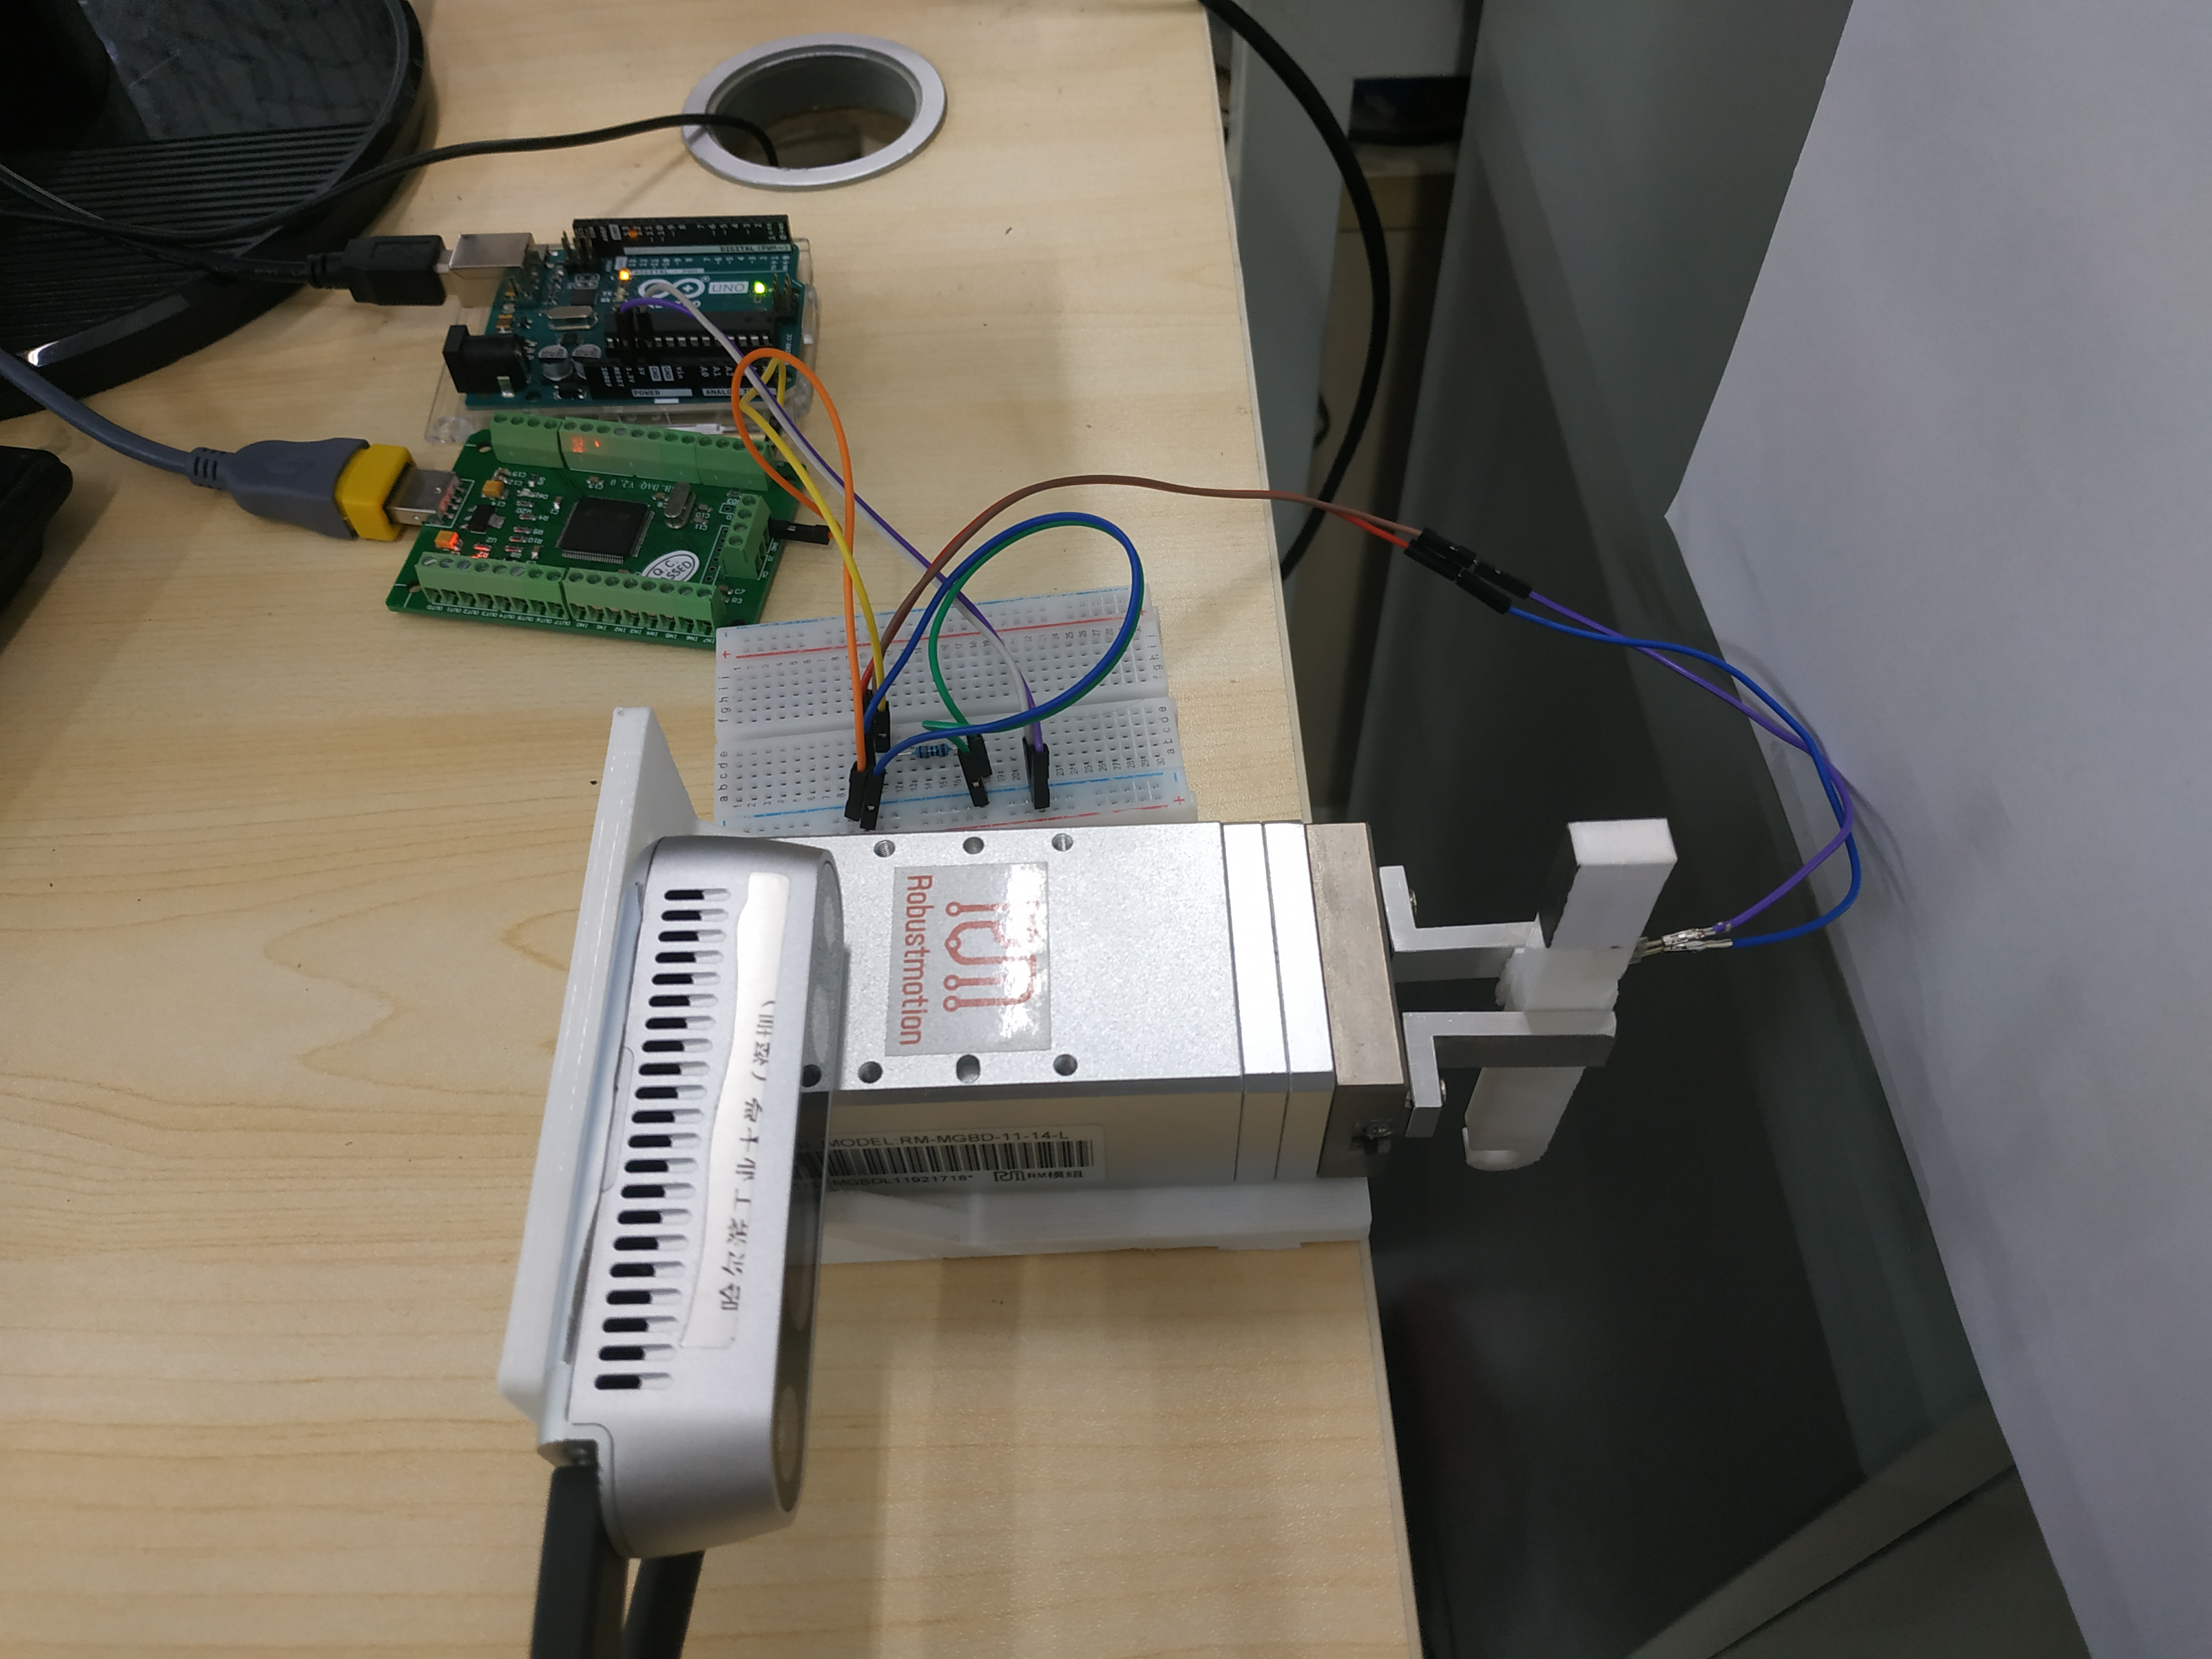
\includegraphics[width=7.2cm]{chapter04/pic/exp-2}
%     }
%   \caption{本项目搭建的实验平台}
%   \label{fig:experiment}
%   \vspace{-0.3cm}
% \end{figure}

\section{压力传感器的校准}
实验使用的压力传感器类型为:宇博智能 RFP601 型薄膜压力传感器,量程为500g,
是一款压阻式单点压力传感器, 响应时间为微秒级。
图 \ref{fig:4-2} 所示是该传感器的压阻特新曲线图。
实验使用的信号采集器为恒凯 USB 数据采集卡,
提供 12 位 AD采集通道支持 $0\sim 3.3V$ 模拟输入,最高采样频率可达 100Ksps。

\begin{figure}[!ht]
  \centering
  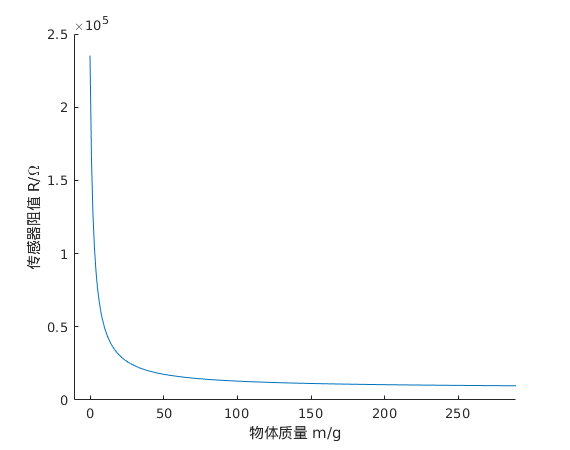
\includegraphics[width=12cm]{chapter04/pic/4-2}
  \caption{薄膜式压力传感器压的阻特性曲线}
  \label{fig:4-2}
  \vspace{-0.3cm}
\end{figure}

该传感器的电阻和压力曲线可近似用反比例函数表示。即式(\ref{equ:4-1})。
设计如图\ref{fig:4-3}所示电路图,图中电源电压为 3.3V, $R_0$ 为固定电阻,
压敏电阻 $R$ 为传感器。通过 A 点电压值可以计算传感器的阻值,即式(\ref{equ:4-2})。
代入式(\ref{equ:4-1})即可得到压力与 A 点电压的关系式(\ref{equ:4-3})。

\vspace{-10pt}
\begin{equation}
  \label{equ:4-1}
  R = \frac{{k'}}{{m + c'}} + a'
\end{equation}
\vspace{-30pt}

\begin{equation}
  \label{equ:4-2}
  R = (\frac{V}{u} - 1) \cdot {R_0}
\end{equation}
\vspace{-30pt}

\begin{equation}
  \label{equ:4-3}
  m = \frac{{c - ku}}{{au - 1}}
\end{equation}

式中 $R_0$ 为固定电阻阻值 $(\Omega )$ , R 为压敏电阻阻值 $(\Omega )$ ,
$m$ 为传感器受到的力 $(g)$ , $V$为电源电压, $u$ 为 $A$ 点电压值,
$a'$, $c'$, $k'$, $a$, $c$ , $k$ 均为与电阻 $R$ 有关的常数。

\begin{figure}[!ht]
  \centering
  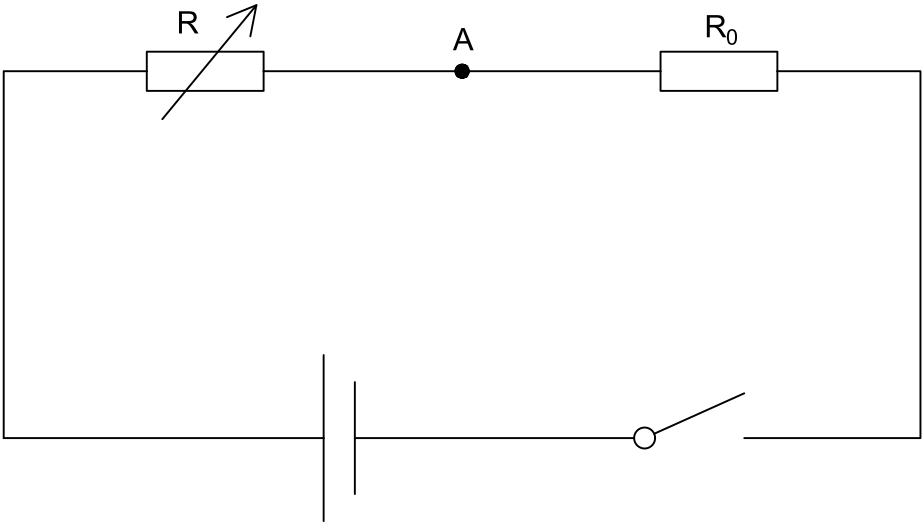
\includegraphics[scale=0.4]{chapter04/pic/4-3}
  \caption{数据采集电路图}
  \label{fig:4-3}
  \vspace{-0.3cm}
\end{figure}

由式(\ref{equ:4-3})可知, $u$ 趋近于 0 时传感器精度过低,对受力响应过大;
$u$ 趋近于 $cV$ 时传感器灵敏度过低。适当调整固定电阻的阻值可以改善传感器效果,
经实验确定该项目拟用阻值为 $R=10k\Omega$ 的固定电阻。

多次测量不同压力下 A 点的电压值,绘制散点图如图\ref{fig:4-4}所示,利用 Matlab 进行
拟合,拟合结果确定式(\ref{equ:4-3})中的参数为
$c = − 6.431$ , $ k = 10.72 $ , $a = 0.4967$ ,置信概率为 $95\%$ 。

\begin{figure}[!ht]
  \centering
  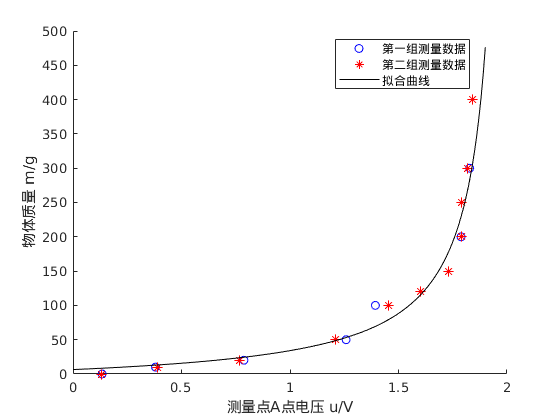
\includegraphics[width=13.5cm]{chapter04/pic/4-4}
  \caption{采集数据散点图与拟合图}
  \label{fig:4-4}
  \vspace{-0.3cm}
\end{figure}

\section{高速夹爪的伺服控制与力控}
实验中使用的夹爪为增广智能科技 RM-MGBD--11-14-L 微型伺服夹爪。
控制器与夹爪通信时间约为 5ms, 即发送运动信息和读取夹爪位置需要 5ms 的时间,
由于力控不需要夹爪位置反馈, 故伺服周期应大于 5ms,
考虑到读取传感器数据和程序运行等需要一定的时间, 我们将伺服周期设为 8ms。

在力控实验中经过多次参数调整后,我们最终采用的 PD 控制器参数为
$k_p = 0.0008$ , $k_i = 0.0004$, $k_d = 0.0008$ 。
下面图\ref{fig:150}至图\ref{fig:sin_x}分别展示了使用改良PD控制算法后系统的输出信号
相对恒定输入信号和正弦输入信号的跟踪效果。



% \begin{figure}[!h]
%   \centering
%     \subfloat[压力变化曲线]{
%       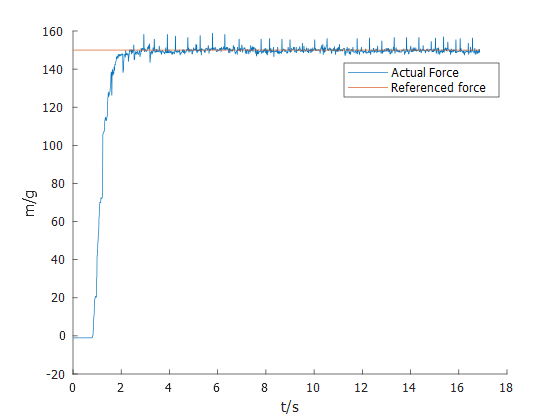
\includegraphics[width=7.2cm]{chapter04/pic/150}
%     }
%     \hspace{0pt}
%     \subfloat[夹爪位置信号]{
%       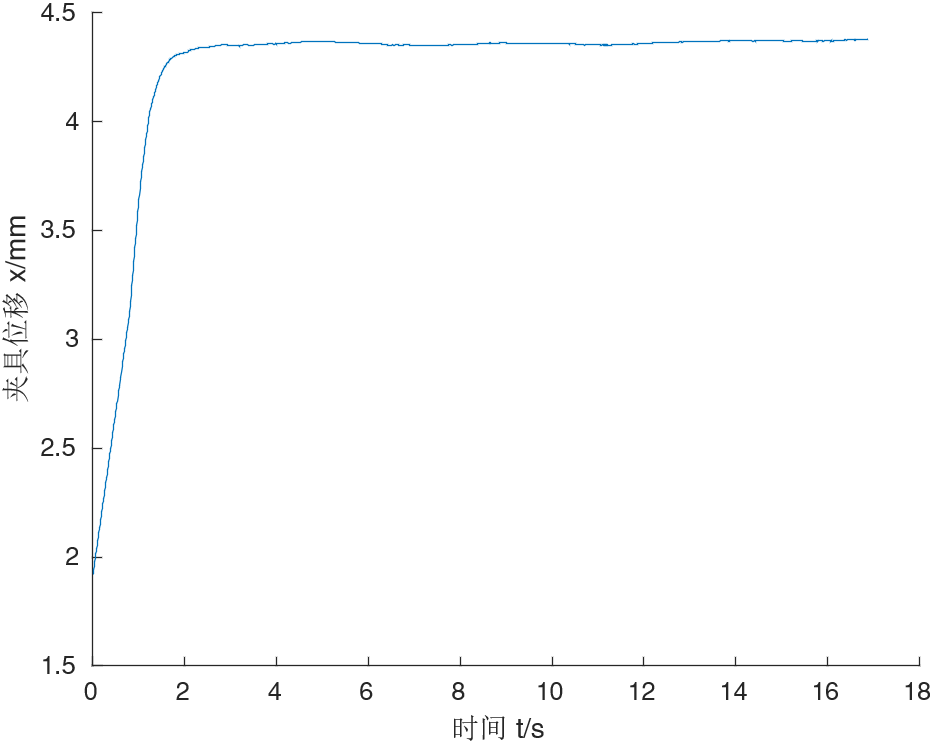
\includegraphics[width=7.2cm]{chapter04/pic/150_x}
%     }
%   \caption{\label{fig:4-5}阶跃信号下的压力和夹爪位置信号曲线}
%   \vspace{-0.3cm}
% \end{figure}

% \begin{figure}[!ht]
%   \centering
%   \includegraphics[scale=0.70]{chapter04/pic/4-5}
%   \caption{PID控制下系统阶跃响应}
%   \label{fig:4-5}
%   \vspace{-0.3cm}
% \end{figure}

图\ref{fig:150}可以展示了 改进后的控制器在阶跃输入信号下的控制效果。
最终压力均值保持在期望值 150 g左右,输出信号的波动主要原因是传感器误差,
波动范围在可接受范围内。
调节时间约为 2s ,这并不影响我们的实验的控制效果,因为实际实验中,
初始状态下夹爪是抓紧工具的,而在运动过程中压力变化虽然很频繁但是增量不大,
所以实验过程中压力信号的改变幅度不会过大,压力信号与实际压力值相差也较小,
因此图示的调节时间是可以接受的。

\begin{figure}[!ht]
  \centering
  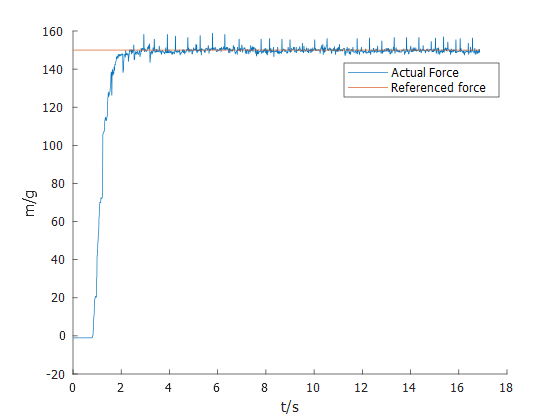
\includegraphics[width=11cm]{chapter04/pic/150}
  \caption{\label{fig:150}
    阶跃信号下传感器采集的压力信号曲线}
  \vspace{-0.3cm}
\end{figure}

图\ref{fig:150_x}展示了在这一过程中控制器对夹爪发送的位置命令,
可以看到位置信号和压力信号的变化趋势趋于一致,
而且在压力值到达150g附近时位置命令保持稳定,只有轻微的振动,
这也说明了压力的波动是由于传感器造成的。

\begin{figure}[!ht]
  \centering
  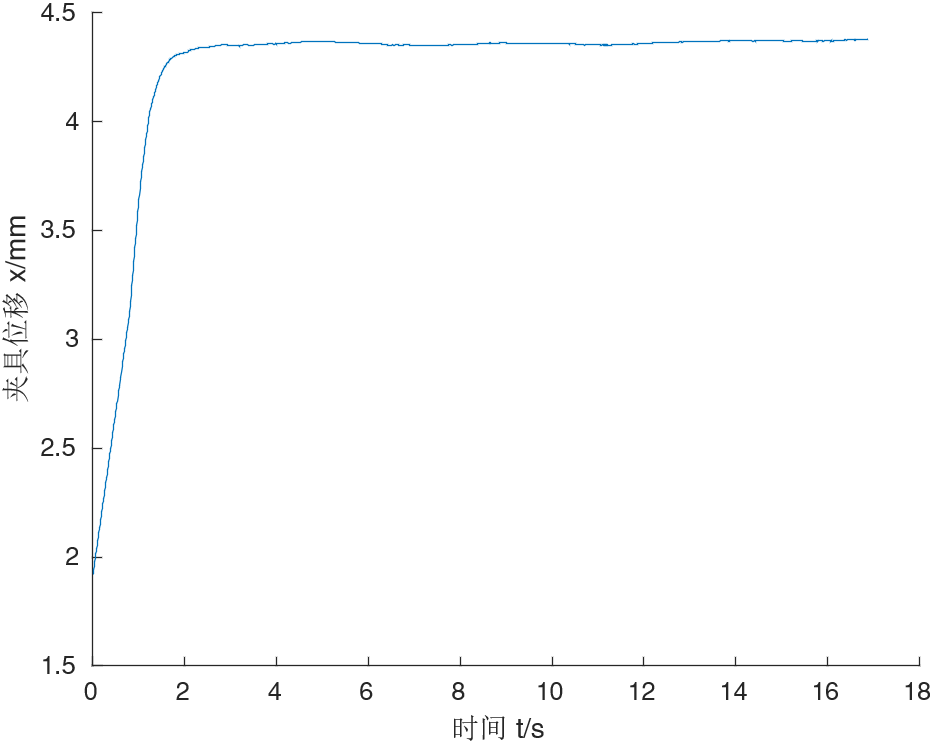
\includegraphics[width=10cm]{chapter04/pic/150_x}
  \caption{\label{fig:150_x}
    阶跃信号下夹爪位移信号曲线}
  \vspace{-0.3cm}
\end{figure}



% \begin{figure}[!h]
%   \centering
%     \subfloat[压力变化曲线]{
%       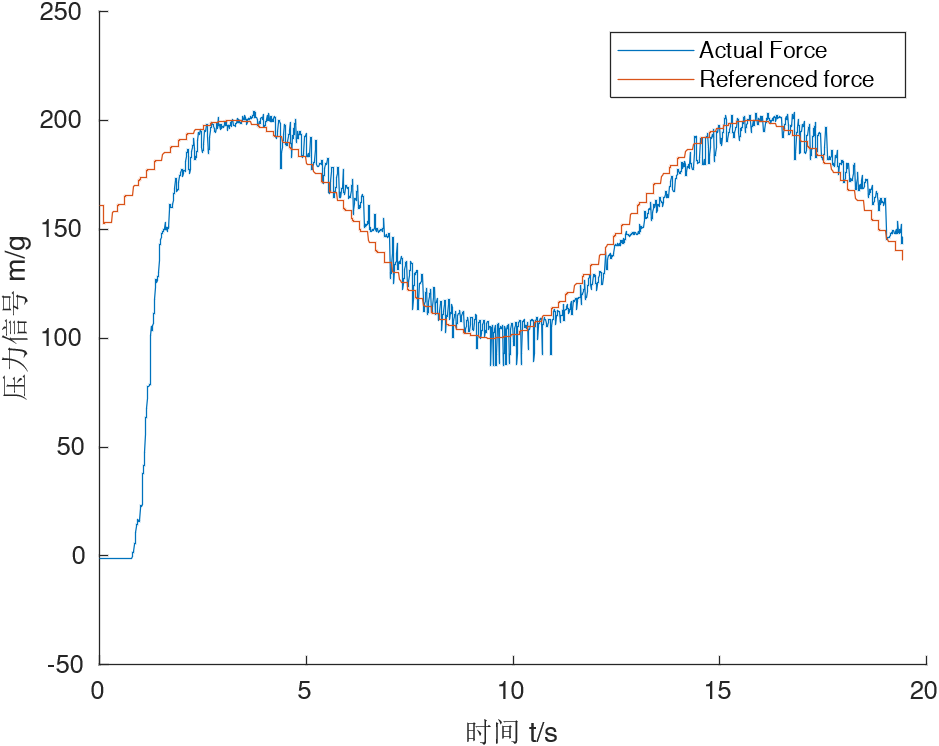
\includegraphics[width=7.2cm]{chapter04/pic/sin}
%     }
%     \hspace{0pt}
%     \subfloat[夹爪位置信号]{
%       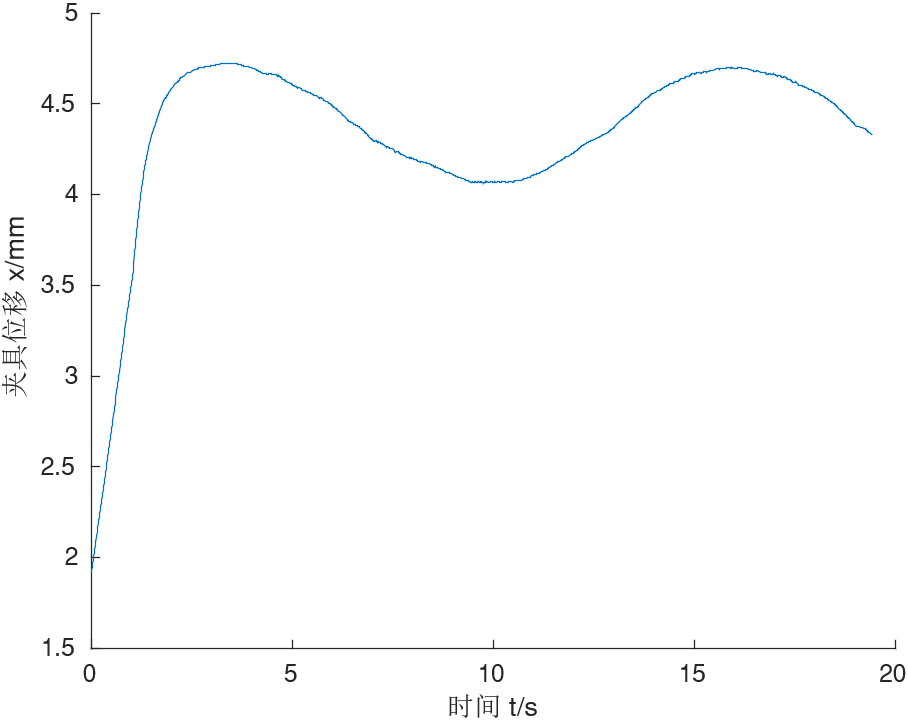
\includegraphics[width=7.2cm]{chapter04/pic/sin_x}
%     }
%   \caption{\label{fig:4-6}正弦信号下的压力和夹爪位置信号曲线}
%   \vspace{-0.3cm}
% \end{figure}

% \begin{figure}[!ht]
%   \centering
%   \includegraphics[scale=0.70]{chapter04/pic/4-6}
%   \caption{PID控制下输出量对正弦信号的跟踪性能}
%   \label{fig:4-6}
%   \vspace{-0.3cm}
% \end{figure}

从图\ref{fig:sin}可以看出在信号持续变化的情况下 PD 控制器的控制效果也符合预期。
长时间的控制下,虽然传感器误差会有一定的波动,但是系统保持稳定,
实际压力均值持续跟随正弦输入信号,没有明显的误差,输出信号的波动范围在可接受范围内。
同理调节时间并不影响我们的实验的控制效果。
结合这两个实验可以说明 PD控制是可以满足我们的控制需求的。

\begin{figure}[!ht]
  \centering
  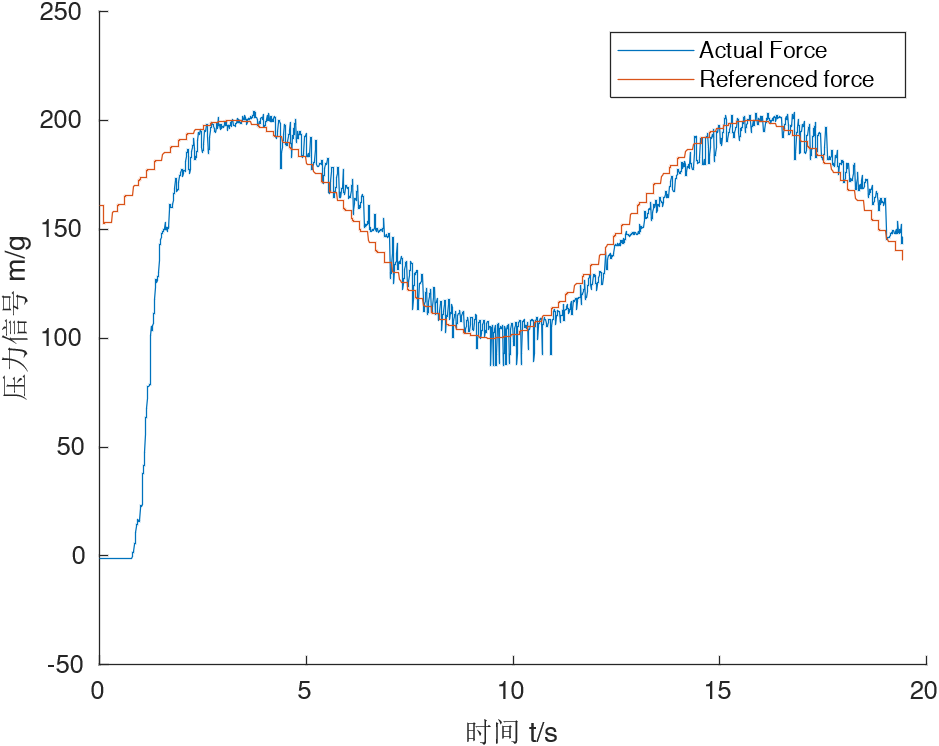
\includegraphics[width=10cm]{chapter04/pic/sin}
  \caption{\label{fig:sin}
    正弦输入信号下传感器采集的压力信号曲线}
  \vspace{-0.3cm}
\end{figure}

图\ref{fig:sin_x}展示了在该过程中控制器的位置指令的变化曲线,
可以看到位置信号和压力信号的变化趋势趋于一致。
同样,这也说明压力信号中的偶尔出现较大的偏差是由于传感器测量误差导致的,
应该在PD控制器中添加滤波算法,以减小或排除偶然误差。
%位置信号不是严格的正弦信号, 这是因为传感器采集的电压信号转化为压力信号不是线性的。
%所以在不同压力大小下产生同样压力差所需的位移大小不同,
%在位置信号图上,压力在极大值和极小值附近的变化幅度有差异。

\begin{figure}[!ht]
  \centering
  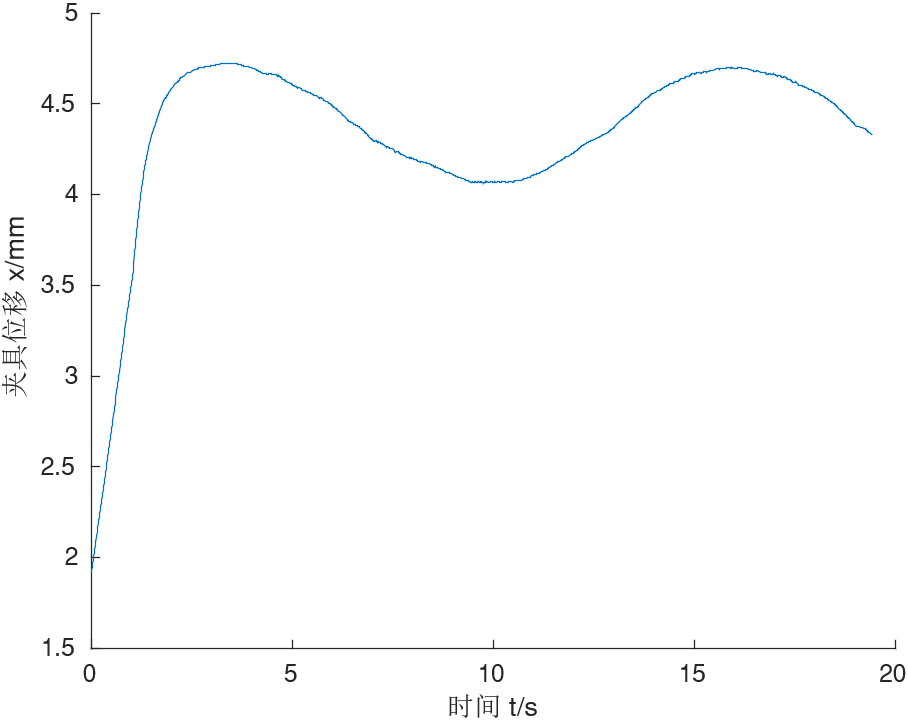
\includegraphics[width=10cm]{chapter04/pic/sin_x}
  \caption{\label{fig:sin_x}
    正弦输入信号下夹具的位移信号曲线}
  \vspace{-0.3cm}
\end{figure}

\section{边缘检测与相机标定}
本项目中使用的相机型号为Realsense D435。相机固定在机械臂末端,相对于夹爪位置固定,使用彩色相机测量物体的位置。
由于操作过程中机械臂不发生运动,
所以物体相对于相机坐标系的变化即为相对于基坐标系的变化。
Realsense相机获得的图片是每个像素点的BGR信息组成的矩阵,
每个像素点均以距离左上角的像素距离来定位。
我们实际需要获得的是图片上特定距离与实际物体的长度的对应关系,
即每个像素点与实际长度单位的关系, 这需要通过标定相机来确定。

本项目使用如图\ref{fig:src}所示的标定物进行标定。
图中黑色区域长度为$20mm$, 将标定物放在被控物体需要安放的位置,
通过测量相机返回的图片中黑色区域的像素点宽度来校准相机。
可以通过将相机返回的图片转化为灰度图,进而使用Canny边缘检测来识别图片中黑色区域的边缘,
如图\ref{fig:canny}所示为识别出来轮廓, 再利用Hough变换可以计算图中直线的端点位置。
依次遍历各条直线,计算其斜率并筛选水平的直线。将各条水平直线之间的高度差最大值记为黑色区域的像素长度,
这样就能计算出每个像素点宽度对应的实际长度。

% \begin{figure}[!h]
%   \centering
%     \subfloat[相机标定原图]{
%       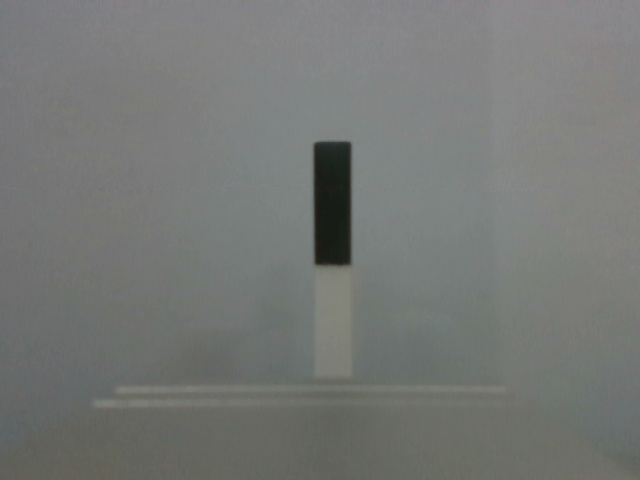
\includegraphics[width=7.2cm]{chapter04/pic/src}
%     }
%     \hspace{0pt}
%     \subfloat[边缘检测图]{
%       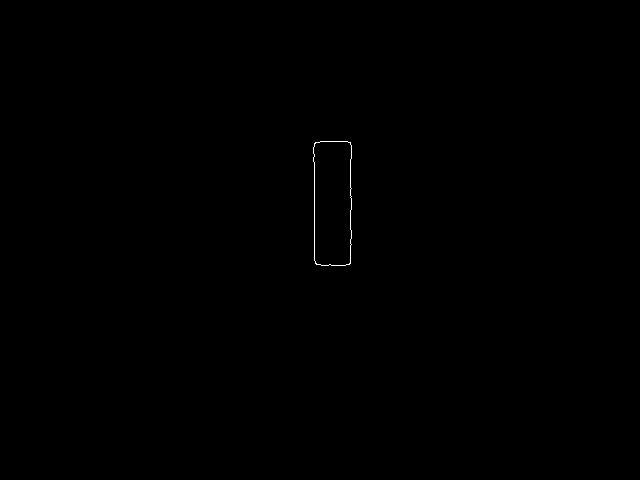
\includegraphics[width=7.2cm]{chapter04/pic/canny}
%     }
%   \caption{夹具位移及受力曲线图}
%   \label{fig:src}
%   \vspace{-0.3cm}
% \end{figure}

相机标定完成后,需要对抓取物体进行定位。本项目中在实验开始前,选取物体静止时上边缘高度记为坐标轴原点,
向下为正方向。识别物体上边缘的方法为:将物体图片转化为灰度图,利用Canny识别边缘,再利用Hough变换计算直线端点位置,
最后根据直线斜率和高度,筛选像素点位置最低的水平直线,即物体上边缘,此直线的高度减去原点高度即为当前时刻物体的位置。

\begin{figure}[!ht]
  \centering
  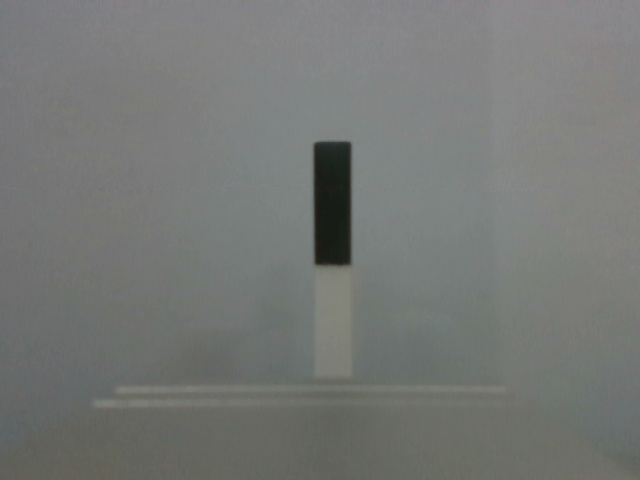
\includegraphics[width=10cm]{chapter04/pic/src}
  \caption{\label{fig:src}
    相机采集的图片}
  \vspace{-0.3cm}
\end{figure}

\begin{figure}[!ht]
  \centering
  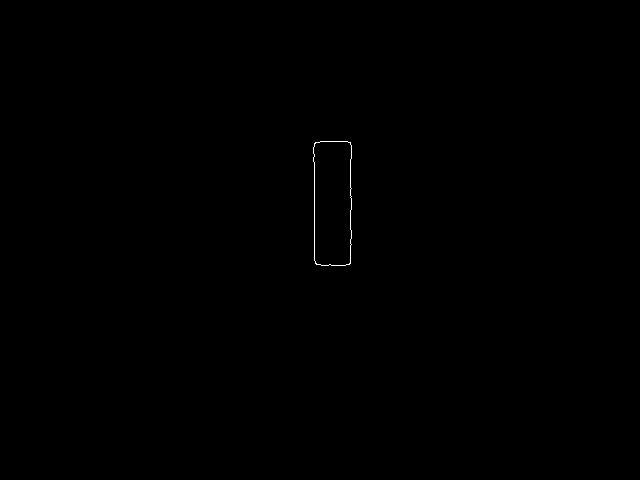
\includegraphics[width=10cm]{chapter04/pic/canny}
  \caption{\label{fig:canny}
    Canny边缘检测提取的边缘信息}
  \vspace{-0.3cm}
\end{figure}

\section{实验结果及其分析}
完成上述实验准备后, 我们进行了多组实验,
实验中采用的自适应控制参数如表\ref{tab:exp}所示。

\begin{table}[!h]
\centering
\caption{实验中自适应控制参数取值表\label{tab:exp}}
\begin{tabular}{@{}ccccc@{}}
\toprule[1pt]
 \makebox[2.5em][c]{$k$}        & \makebox[2.5em][c]{$\lambda$}  &
 \makebox[2.5em][c]{$\alpha_a$} & \makebox[2.5em][c]{$\alpha_c$}  &
 \makebox[2.5em][c]{$\alpha_c$} \\ \midrule

6        &  6        & 20      &  20     &  20    \\
\bottomrule[1pt]
\end{tabular}
\end{table}

在改变被控物体质量, 其他参数不变的情况下进行在手操作实验, 实验结果并不理想。
总体表现为控制器反应过慢, 在物体开始下落后控制器并未能及时调整控制参数,
从而导致物体超过期望位置后夹具才开始阻止物体下落。
其中一次在手操作过程中, 物体的下落曲线和夹具压力信号曲线分别
如图\ref{fig:h}和图\ref{fig:f}所示。

\begin{figure}[!ht]
  \centering
  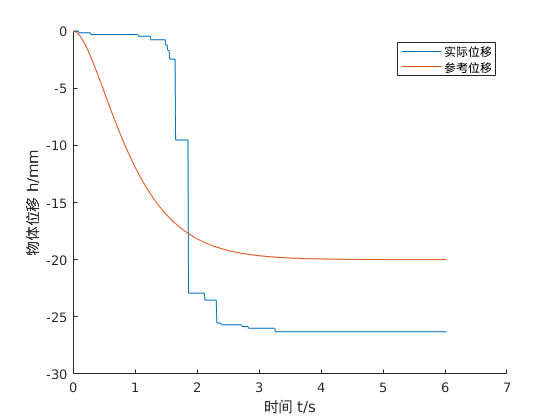
\includegraphics[width=12cm]{chapter04/pic/h}
  \caption{\label{fig:h}
    在手操作实验过程中物体的下落曲线}
  \vspace{-0.3cm}
\end{figure}

\begin{figure}[!ht]
  \centering
  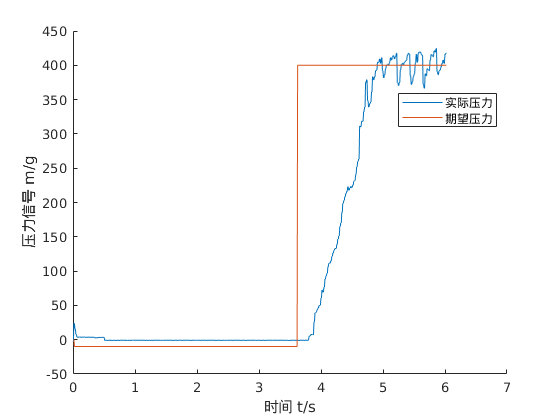
\includegraphics[width=12cm]{chapter04/pic/f}
  \caption{\label{fig:f}
    在手操作实验过程中传感器压力信号曲线}
  \vspace{-0.3cm}
\end{figure}

% \begin{figure}[!h]
%   \centering
%     \subfloat[物体下落曲线]{
%       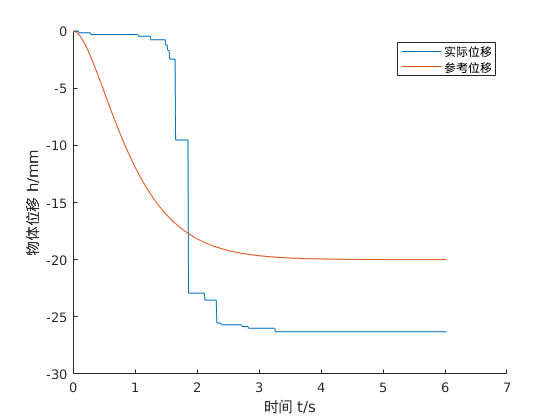
\includegraphics[width=7.2cm]{chapter04/pic/h}
%     }
%     \hspace{0pt}
%     \subfloat[夹具压力信号曲线]{
%       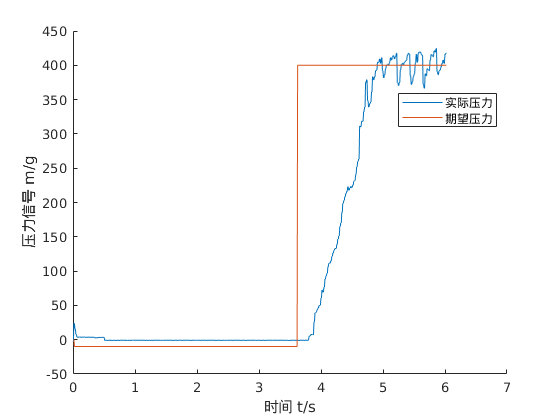
\includegraphics[width=7.2cm]{chapter04/pic/f}
%     }
%   \caption{实验中物体运动和夹具压力信号曲线}
%   \label{fig:fh}
%   \vspace{-0.3cm}
% \end{figure}

从图\ref{fig:h}中可以看出实验效果较差。
物体在开始时缓慢下落, 控制器并未做出反应, 而当物体快速下落一段时间后,
控制器才向夹爪发送较高的压力信号, 但是这时物体已经超过了期望位置。
还存在的一个问题是压力信号变化过大, 每次压力信号发生变化时直接从最小值增加到最大值。

由于实验准备不充分, 导致设计时可能忽略了部分影响因素。
但就目前的实验状况而言, 我们可以总结出导致实验失败的部分原因:
一是夹具容易晃动导致夹爪和物体接触不完全,
导致夹爪在形同的位置时物体的运动状态可能不同;
图中传感器测得的实际压力为0时, 物体开始未发生滑动, 但约1s后物体缓慢下降。
二是控制参数调整不合理, 图\ref{fig:f}中压力信号变化过大就是这个原因导致的。
三是控制参数饱和积分饱和的问题, 自适应控制器中, 控制参数单次的调整量与误差有关,
在实验开始时, 压力信号为0但物体还未开始下落, 此时控制器还在对参数进行误差累加,
导致物体开始下落后, 控制器需要一定时间来抵消饱和误差, 之后才开始产生反向信号。



\section{本章小结}
为验证单自由度机器人手进行被动在手操作的实现方法设计了一套实验方案。
分析了压力传感器输出特性,设计测量电路,校准了传感器。
完成了高速夹爪的伺服控制和力控实验。
最后进行了实验并分析实验结果,
论证了使用模型参考自适应控制算法实现物体在手操作的合理性。

